%TEX TS-program = xelatex
\documentclass[11pt,twoside]{article}
\usepackage[margin=2.54cm]{geometry} % set margins to 1 inch all the way around
\usepackage{fontspec}
	\defaultfontfeatures{Ligatures=TeX}
%	\newcommand{\lmr}{\fontfamily{lmr}\selectfont} % Latin Modern Roman
%	\setmainfont{Birka LT Pro}
    \setmainfont[Mapping=tex-text]{Kepler Std Light}
    \setsansfont[Mapping=tex-text]{Myriad Pro}
    \setmonofont[Scale=MatchLowercase]{Anonymous Pro}
\renewcommand{\ttdefault}{mf} % this makes the monospace font the default one used to what I specified
\usepackage{emptypage} % this keeps footers off the blank page
% set line spacing to 1.5
\usepackage{setspace}
\onehalfspacing 
\setlength{\parindent}{0pt} % don't indent paragraphs globally

\usepackage{titlesec}
    \titleformat{\section}{\Large\bfseries\sffamily}{\thesection}{1em}{}
    \titleformat{\subsection}{\large\bfseries\sffamily}{\thesubsection}{1em}{}
    \titleformat{\subsubsection}{\normalsize\bfseries\sffamily}{\thesubsubsection}{1em}{}

% set up indexing for all the acronyms
\usepackage{makeidx}
    \makeindex
\usepackage[acronym,toc]{glossaries}
    \makeglossaries
\usepackage{graphicx}   % this handles the non-native charts
%\usepackage[sectionbib]{chapterbib} % this handles references per chapter
% this handles the risk equation -- may not be necessary
%\usepackage{amsmath}
%\usepackage[font=sf, labelfont={sf,bf}, margin=1cm]{caption}
\usepackage[font=small]{caption}
\PassOptionsToPackage{hyphens}{url}\usepackage{hyperref}
\renewcommand{\UrlBreaks}{\do\/\do\a\do\b\do\c\do\d\do\e\do\f\do\g\do\h\do\i\do\j\do\k\do\l\do\m\do\n\do\o\do\p\do\q\do\r\do\s\do\t\do\u\do\v\do\w\do\x\do\y\do\z\do\A\do\B\do\C\do\D\do\E\do\F\do\G\do\H\do\I\do\J\do\K\do\L\do\M\do\N\do\O\do\P\do\Q\do\R\do\S\do\T\do\U\do\V\do\W\do\X\do\Y\do\Z} % this handles breaking URLS smartly
\usepackage{enumitem}

\setcounter{tocdepth}{2} % table of contents include subsections

\usepackage{listings} % handle code formatting for the appendix

% modify footer to include disclaimer
\usepackage{fancyhdr}
\pagestyle{fancy}
\fancyhead{}
\renewcommand{\headrulewidth}{0pt}
\fancyfoot{}
% \fancyfoot[LO,RE]{\small\textit{\textsc{CSC} Confidential. For Internal Distribution Only.}}
\fancyfoot[LE,RO]{\thepage}

\DeclareMathSizes{10}{18}{12}{8}

\usepackage{wrapfig} % wrap text around the picture in the author bio



\begin{document}
    %!TEX root=index.tex
\begin{titlepage}
    \vspace*{\fill}
    \begin{center}
        \textbf{\Large Christopher Keller}\\[1cm]
        \textit{A Big Data Approach To ClimatEdge\texttrademark{}}\\ [.5cm]
        CSC NPS Solution Leadership Institute\\ [.5cm]
        %\today
        March 28, 2014
    \end{center}
    \vspace*{\fill}
\end{titlepage}

    \cleardoublepage
    \tableofcontents
    \pagenumbering{roman}
    \cleardoublepage
    %!TEX root=index.tex
\newacronym{cse}{CSE}{Certified Solution Executive}
\section{Executive Summary}
\textsc{CSC's} ClimatEdge\texttrademark{}\index{ClimatEdge} offering is focused on providing probabilistic climate analytics using public government data sets. By using various algorithms, both proprietary and public, \textsc{CSC} plans to offer its customers a distinct advantage by allowing strategic business decisions to be made based on probabilistic outlooks in climate and extreme weather. Planned offerings for the general insurance industry include the probability of future tornado, hail, or flood occurrences in a particular geographic grid cell, as well as hail activity in the recent past.\\

This paper focuses on contrasting the tornado and flood offerings with respect to the attributes associated with big data: velocity, volume, and variety. The hail offering is similar enough in variety to tornado and in volume to flood, that analyzing it separately does not add further insights or value. The computation of tornado probabilities involves running a published algorithm against a relatively small amount of structured data on modest hardware. In short, it does not meet the criteria for big data. Flood probabilities, on the other hand, require substantially larger and more diverse data such as newspaper reports, hydrologic data from stream gauges, and parcel information in addition to rainfall and other climate data. In contrast to the tornado analytic, it does meet several criteria for big data. The minimal platform capable of delivering the tornado probabilities is not capable of offering flood probabilities. Without an investment in big data technology and expertise, the range of ClimatEdge\index{ClimatEdge} offerings will be limited.\\

Next, a reference framework implementation is presented that will allow tornado, flood, and future ClimatEdge\index{ClimatEdge} offerings to scale in processing both large and complex data sets, thus enabling a wider variety of business cases to be developed into offerings. The most important framework characteristics are flexibility in implementation technologies and a loose coupling between the layers. There does not exist a single application or technology capable of addressing every offering scenario, therefore a collection of specific technologies that can be integrated together is presented. As technologies evolve, the goal is to be able to replace any one piece of technology without overly affecting the other layers.\\

Finally, three future research ideas around the processing of large data sets are presented. The first relies on a data owner enabling programatic access, but not necessarily analysis, to the data.  The second option focuses on the possible legal implications of results derived from cloning any data sets to local storage. Finally, an approach based on moving the analysis to the provider data center is explored. Each approach has both advantages and disadvantages and is suitable for further research within \textsc{CSC} or as a follow on \gls{cse} thesis.
    \pagenumbering{arabic}
    %!TEX root=index.tex
\newacronym{merra}{MERRA}{Modern-Era Retrospective Analysis for Research and Applications}
\newacronym{html}{HTML}{Hyper Text Markup Language}
\newacronym{sme}{SME}{Subject Matter Expert}
\newacronym{pdf}{PDF}{Portable Document Format}
\newacronym{noaa}{NOAA}{National Oceanic and Atmospheric Administration}
\newacronym{nasa}{NASA}{National Aeronautics and Space Administration}
\section{Introduction}
Across the globe, the big data movement is changing how meteorologists are storing and analyzing data in response to global events. For example, efforts by the Korean Meteorological Administration are underway to upgrade the ability to predict weather patterns and the severity of weather events across the South Korean peninsula. IBM is engaged in similar work in Rio de Janeiro in preparation for the 2014 summer Olympics, with goals of accurately predicting short term weather \cite{rwe}. Moving past short term predictions, what if the vast repositories of weather and climate data could be collected, stored, and analyzed to produce probabilities of catastrophic events months, not weeks, in advance?\\

In 2012, \textsc{CSC's} ClimatEdge\texttrademark{}\index{ClimatEdge} service was developed to explore the commercial potential of publicly held climate and weather data. The initial offering focused on forward looking climate reports for commodities markets. The reports were written using a cursory qualitative analysis of the NASA \gls{merra} data with commentary by subject matter experts in climate sciences. The monthly reports included Global Agriculture, Global Energy, Sugar and Soft Commodities, Grain and Oilseeds, and Energy/Natural Gas \cite{climatedgeurl}. Interviews conducted with individuals associated with the original ClimatEdge\index{ClimatEdge} offering described a number of lessons learned and decisions that led to a strategy shift to a quantitative product for the next version [personal communication, 2013]. Potential customers were less interested in commentary on qualitative analysis than originally thought. Along with other factors, the ClimatEdge\index{ClimatEdge} team made the decision to focus on quantitative analysis utilizing existing CSC sales channels.\\

During the 2012 calendar year, the United States had eleven separate weather events where losses totaled more than one billion dollars each, making it the third highest loss year due to natural catastrophes since 1980 [\textsc{CSC} communication from the \gls{noaa}, 2013]. With premiums increasingly unable to cover losses incurred from extreme weather events, the overall profitability of the insurance industry is at risk. With products such as POINT IN  and Exceed, \textsc{CSC} has significant sales inroads with the general insurance industry \cite{point_in} \cite{exceed}. With established channels, the general insurance industry became a prime target for the second version of ClimatEdge\index{ClimatEdge}.\\

In order to understand offerings for general insurance, the business model must be explored. The following equation can be applied to the general insurance industry: 
\begin{equation*}
    Risk = Impact \cdot Probability
\end{equation*}
\textsc{CSC} recognized that without a substantial quantitative update, ClimatEdge\index{ClimatEdge} could not address the probability of events occurring, thus the overall risk could not be established. With a wealth of publicly available climate data from agencies such as \gls{noaa} and the \gls{nasa}, \textsc{CSC} realized a business opportunity existed. A ClimatEdge\index{ClimatEdge} offering based on quantitative analysis of publicly available data targeted towards minimizing risk for the general insurance industry would be a natural fit. The next step was to develop a technical approach to retrieving, storing, and analyzing the wealth of available data. 
\subsection{Hypothesis}
Without investing in and developing a scalable solution for big data \index{big data} storage and analytics, ClimatEdge\index{ClimatEdge} offerings will be limited to markets served by either qualitative analysis or quantitative analysis against small well-structured data sets. In order to analyze the larger and more structurally complex climate data sets, a framework of scalable technologies will need to be developed that can address both simple and complex offerings of any size. With the proper framework in place, \textsc{CSC} can offer solutions derived from analytics on data having one or more of the following big data characteristics: velocity, volume, or variety to an ever increasing number of industries.\\
 
Two contrasting ClimatEdge offerings will be explored that illustrate the different requirements necessary to store and analyze the requisite climate data. The first offering is shown to not be representative of a big data problem and is solvable by simple technology. The second offering has all the characteristics of a problem in need of a big solution. A flexible framework is then proposed that illustrates how to store and process larger and more complex data sets, such as those seen in the second offering.
\subsection{Offerings}
The large number of severe weather events in 2012, such as tornados, floods, and other natural catastrophes, caused \$160 billion dollars worth of damage in the United States \cite{stalder}. This is near the total of the previous ten years combined. Throughout that same ten year period, insured losses totaled over \$65 billion. Tornados, while a worldwide phenomenon, occur with greater frequency in the United States due to the meeting of cold Canadian air with low-level moisture from the Gulf of Mexico. Losses from these severe storms alone have accounted for more than half of all insured catastrophe losses since 1990 \cite{lloyds}. Several presentations at the Extreme Weather Congress in January 2013 focused on flooding as a prime source of damage. In the United States, floods are the most common natural disaster and average about six billion in damages each year and while the National Flood Insurance Program provides limited coverage to homeowners and businesses that qualify, a sizable secondary insurance market exists \cite{hope}. Globally, floods rank only behind earthquakes as the world's costliest natural disasters \cite{li}. \textsc{CSC's} Data Services group, in conjunction with industry analysts and other internal groups, has identified several opportunities in which an updated ClimatEdge\index{ClimatEdge} offering can benefit the general insurance industry [personal communication, 2013]:
\begin{itemize}
    \item probability of future tornado occurrence
    \item probability of future hail occurrence \& recent forensics
    \item probability of future global and domestic flood occurrence
\end{itemize}
This paper examines the tornado and flood probability analytics as having contrasting requirements at either end of the attribute scale associated with big data. The analytics necessary for producing a hail offering are an offshoot of the tornado algorithm and the data sets required are also similar in complexity to the tornado sets. A detailed examination of the hail offering would therefore, not yield significant additional insight as compared to tornado and flood offerings.
    %!TEX root=index.tex
\newacronym{acm}{ACM}{Association of Computing Machinery}
\newacronym{ncdc}{NCDC}{National Climatic Data Center}
\newacronym{soi}{SOI}{Southern Oscillation Index}
\newacronym{tvs}{TVS}{National Tornado Vortex Signature}
\newacronym{nosql}{NoSQL}{Not only SQL}
\newacronym{xml}{XML}{Extensible Markup Language}
\section{Use Cases}
Two offerings with sufficiently different data and processing requirements are tornado and flood. While both are similar in  respect that the objective is to produce a probability of occurrence for any given geographical point in the coverage area, the technology required to accomplish this varies greatly. A primary carrier of property and casualty insurance would be very interested in knowing the probability of natural catastrophes in geographical areas in which they have a large customer base. Having accurate predictions of seasonal event probabilities, months in advance, constitutes a significant business advantage over competitors when issuing or renewing premiums. \\

In a \textsc{CSC} meeting with Novarica, an insurance industry consulting group, a scenario was laid out in which insurance underwriters would be given access to an additional data feed which housed catastrophic weather event probabilities [personal communication, 2013]. This feed would be ingested into current toolsets, which assist in the creation of appropriate terms and rates offerings for their customers. Catastrophic weather events, successfully predicted months in advance, can help the insurance companies balance high risk policies with low risk polices in their overall portfolio, in order to maximize revenue.  Insurance companies need long term predictive outlooks, because existing books of business cannot be changed in the short term.
\subsection{Offerings}
Quantitative predictions for natural catastrophic events such as tornado, hail, or flood can be expressed as a Poisson distribution showing the probability of a given number of events occurring over a fixed interval of time \cite{anderson}. It is possible to represent the resulting Poisson distribution in a number of ways, either textually or graphically. While an interactive \gls{html} geographical map may best present the results visually, the goal is to get the information into a system capable of overlaying it with parcel and policy data, so as to present a complete picture for risk analysis. \textsc{CSC} has two different administration tools for insurance carriers called POINT IN \cite{point_in} and Exceed \cite{exceed} which can handle \gls{xml} input feeds containing the event probabilities for each geographical grid location. For the global flood offering, the Integral software package, also from \textsc{CSC}, will serve the same purpose \cite{integral}.
\subsection{Big Data}
In a guest \gls{acm} \index{ACM} blog post, Michael Stonebraker gives four detailed definitions to the term big data\index{big data}\cite{stonebraker}.  Big data is classified as having one of the following attributes: velocity, volume, or variety.  Velocity describes the frequency at which data is expected to arrive, either pushed or pulled. Volume is simply the size of the data sets to be ingested, stored, and processed. Variety describes the various heterogeneous sources and formats which comprise the data sets. A big data label can therefore be applied to a data set having  one or more of these attributes.\\

The initial input data sets for tornado comprise the following \cite{walker}:
\begin{itemize}
    \item 1 MB of \gls{soi} historical archives \cite{bom}
    \item 100 MB of \gls{tvs} data \cite{hdss}
    \item 1.5 TB of \gls{ncdc} historical tornado report data\cite{ncdc}
\end{itemize}
All of this data is in the public domain and freely available to anyone that has the resources to store and analyze it. A \textsc{CSC} subject matter expert has speculated that there exist variables stored within the three dimensional \gls{merra} archives that can be utilized to further improve prediction by reducing uncertainty [personal communication, 2013]. This additional data would be:
\begin{itemize}
    \item 1.5 TB of \gls{merra} three dimensional historical data \cite{mdisc}
\end{itemize}
Even with data volumes approaching several terabytes for the full effort, tornado prediction does not conform to the criteria for big data because it lacks all three attributes. The incoming data velocity can be based on several factors: how often is the input data available, how frequently is the output generated, and how long it takes to processes the incoming data. The tornado analytic is expected to be generated monthly which means input must be processed at least that often. The \gls{soi} and \gls{tvs} data sets are small enough to be considered noise with respect to the larger \gls{merra} data. Even at several terabytes, \gls{merra} can still fit on one or two hard drives, eliminating the need for more than one system to store all the data.  Although, four data sets will require four different parsers to process and ingest the data, the parsers are fairly straightforward since the data sets are structured with ample documentation. Preliminary tests have shown that processing a single day of \gls{merra} (300MB) and writing into an SQLite flat file takes approximately 20 seconds per variable a modern CPU \cite{keller1}. Taken together, the velocity, volume, and variety of data do not constitute a challenge in the development of the tornado predictive analytic.\\

The \gls{soi} data set is primarily used as an indicator of an El Niño or La Niña trend, which is useful in predictive climate analytics in general. This data set is updated monthly by the Australian Bureau of Meteorology, giving us a baseline for how frequently our \climatedge offerings will be produced. While specific customers may or may not require monthly feeds, the methods will be in place to generate them at that frequency. Generating them more frequently than monthly will not produce substantially different results.\\

The flood analytics require the following initial public domain data sets \cite{walker}:
\begin{itemize}
    \item \gls{nasa} satellite rainfall data
    \item 2.5 TB \gls{merra} soil moisture, atmospheric wind, humidity, and runoff data
    \item streamflow data as available
    \item damage data from previous floods (newspaper, social media, etc) to augment streamflow
    \item satellite data of built structures and inundation
    \item hydrologic response models
\end{itemize}
Recalling the attributes of big data: velocity, volume, and variety, it becomes clear that flood prediction falls into this category more so than tornado data. It is expected that ingesting relevant newspaper and social media data will add a daily component with reports of damage, especially during the various flood seasons. Even without taking into account the global nature of the offering for flood prediction, the satellite rainfall and \gls{merra} data sets will be larger than the corresponding sets in tornado (mainly due to more input variables). Without even addressing existing structures or the hydrologic response models, the entirety of the input data set is larger. Much of the data sets are computer published, leading to structured input, however the media component implies unstructured data. The flood data has greater volume, higher velocity, and wider variety than the tornado analytic and is more representative of a big data problem.\\

As seen in table \ref{qualifiers},  the flood analytic ingests a larger and wider variety of data sets at a faster pace than the corresponding tornado analytic. Although the format and frequency of both analytic offerings are similar, the infrastructure needed to produce those offerings are quite different in scale.
\begin{table}[htbp]
    \centering
    \begin{tabular}{l l l}
        \hline
        Attribute & Tornado & Flood\\ [0.5ex]
        \hline
        data velocity & monthly & daily\\
        data volume &  3 TB+  & 1 PB+\\
        data variety &  4 sets all structured & 6 sets some structured\\
        \hline
    \end{tabular}
    \caption{Big Data Qualifiers}
    \label{qualifiers}
\end{table}
\subsection{Velocity, Volume, and Variety}
The speed at which sets are processed and stored vary with respect to the particular data. Some data sets are generated daily, e.g. \gls{merra}, some are generated monthly, e.g. \gls{soi}, and some require daily parsing, e.g. newspapers, Twitter \index{Twitter}, or other social media. Although the velocity of incoming data varies by type, it is still expected the output analytics for both tornado and flood are generated monthly on a fixed schedule as determined by the specific customer. If a months worth of data can be be pre-processed in a timely manner, there is no reason to move to daily ingestion. Tests were performed on one month of  \gls{merra} (representative of a larger data feed) and shown that on a single 3GHz core, it takes approximately thirty five minutes to parse and store the data, exclusive of retrieval time. It is not expected that monthly retrieval of the structured data sets will present a problem. The unstructured will need to be gathered  on a daily or semi-daily basis in order to stay current. If not retrieved in a timely manner, there is risk of the data disappearing or time spent processing weekly or monthly bulk loads is prohibitive.\\

It is possible to store  all the necessary data required for the tornado analytic on a 1U server with one terabyte drives. Many home computers also fall into this category. In contrast, if we stored four drives of four terabytes each in a 1U server, we would require sixty-four servers  (or 1.5 standard racks) to store one petabyte worth of flood related data. Replicating the data for high availability adds a factor of two or three to those estimates. Clearly, flood data requires capacity that is orders of magnitude greater than that of the tornado data. An important point to take note of, is that the persistent storage of data after pre-processing could be significantly less what is needed to process it. For example, \gls{merra} files are typically 100 to 300 MB in size, depending on whether it is two or three dimensional. These data files contain variables that may or may not be useful in specific offerings. It is possible that out of over thirty variables, only two or three would actually be used which dramatically reduces the amount of persistent data stored and indexed. The data parsers would know which data they need to permanently store and discard the rest. For this reason, it is crucial that the storage used for pre-processing be elastic to save on costs.\\

Between the tornado and flood data, there are nine separate data sets that need to be pre-processed and stored. While the technology and approach to extracting and storing relevant information from each data is similar, they are still distinct processes that must be developed individually. All four data sets for the tornado analytic are structured with well defined approaches for extracting the required data.  A \gls{merra} parser demonstrating variable extraction and storage has been included in the appendix.  The flood analytic also contains several data sets that are well structured and do not present any significant challenge to data extraction on a continual basis. Within the flood analytic, is the unstructured newspaper and associated social media data related to flood reports and damage. This will require a significantly different parsing technology than the structured data and will be the most challenging to develop, implement, and refine.\\

The flood analytic requires data sets with different attributes than that of tornado. The real time nature of newspaper articles and other social media requires daily or semi-daily ingestion. Significant flooding in a key geographic region may require an out of band delivery of the associated analytics.  This information will be reported first by the media in near real time and not seen in the structured feeds until the end of the month. The additional data sets required by the global and domestic flood offering surpass that of tornado by many times. The same storage technology, but not necessarily the same platform, will work for both offerings at different scales. Tornado data is well structured, while flood data is both structured and unstructured. Different algorithms, involving semantic and natural language processing are necessary to effectively parse the variety of feeds associated with flood reporting by the media.  The attributes shown by the flood  data sets map very well to the accepted criteria of big data, while tornado does not. The technology necessary to produce accurate flood analytics are more complex than tornado and at scale.  The expertise developed by building a platform framework capable of generating analytics on both structured and unstructured data will naturally transfer to the next \climatedge offering, as well as other big data projects.
    %!TEX root=index.tex
\section{Reference Big Data Platform}
In order to quantitatively process ever increasing amounts of complex data, we need a service platform capable of performing the following operational layers:
\begin{itemize}
	\item retrieving data updates
	\item storing and indexing for optimal retrieval
	\item data discovery and analytics
	\item presenting real-time and offline results
\end{itemize}
We can represent each layer graphically, building on the layer to its left. 
\begin{figure}[htp]
    \centering
%    \caption*{Data flow by layer}
    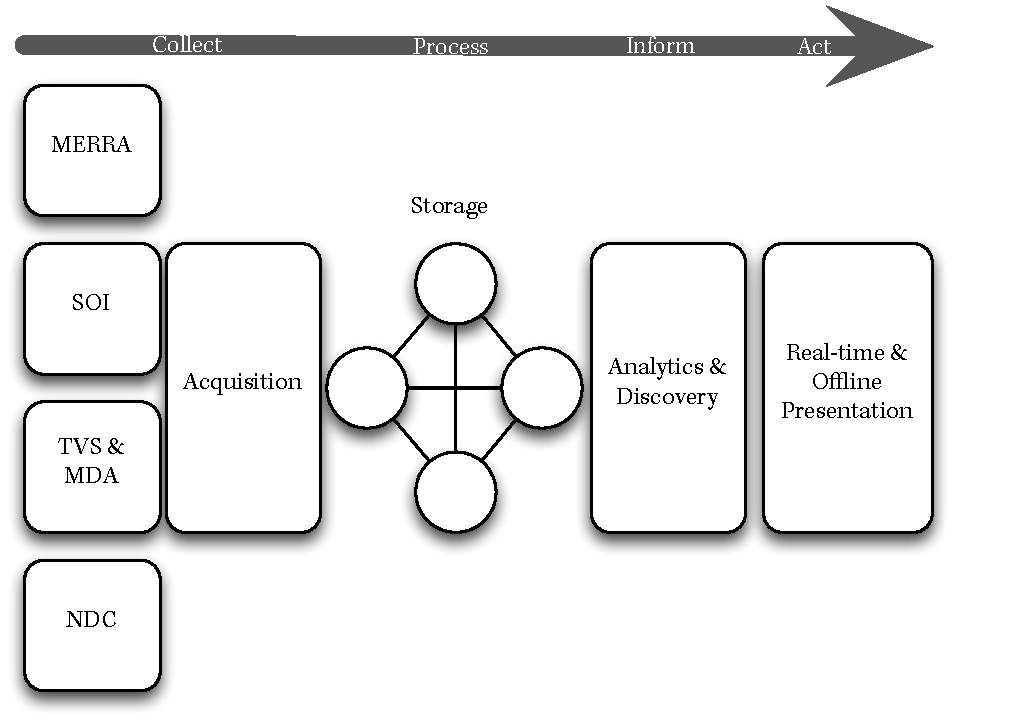
\includegraphics[scale=.75]{dataflow}
\end{figure}

\subsection{Data Acquisition}
As all the data is freely available via standard HTTP requests, we simply need to put together a framework consisting of a repeatable process that polls each website for newly published data and retrieves it. If necessary, the framework can check with the data store to confirm what's new and what's not. Putting together such a framework is a relatively simple systems integration and development task and has plenty of prior art across the industry. I'd recommend the following components:
\begin{itemize}
	\item Three Linux instances to handle retrieval, monitoring, and hosting the source code repository, respectively.
	\item A continuous integration tool, Jenkins or similar, for continually monitoring and notifying the success or failure of the retrieval processes (one per data set). Jenkins will also serve as the means to deploy the most recent code from the code repository onto the server handling the retrieval process. Jenkins is open source and used commonly across the industry for this purpose, resulting in an easily hirable skill set \cite{jenkins}.
	\item A repeatable method, such as Cron, to check and retrieve updated data sets at well defined publication intervals. Jenkins will monitor the success or failure of the cron jobs and notify as needed.
	\item Developed code that contacts each web server and pulls down only the most recent data. If the data sets do not offer a simple means of determining what's recent, this code can query the data store so that it's aware of the last stored data. While we need unique code for each data set, the process of determining what's new and retrieving the code should be very similar across all the data sets. It's likely there will a reusable common library of functionality across each specific implementation. This development is likely to be done in a scriptable environment such as Python or Perl. The languages offer an excellent tradeoff between simplicity, flexibility, and execution speed.
\end{itemize}

\subsection{Storing and Indexing}
Once the data has arrived on the local system, it needs to processed and inserted into the data store. This layer is the heart of any service offering. The data store must have the following characteristics:
\begin{itemize}
	\item Not inherently possess a single point of failure
	\item Horizontally scale (as linearly as possible) in storage and performance
	\item support realtime and batch analytics
\end{itemize}
There exist several technologies in the top level Apache Hadoop project, one being Cassandra\index{Cassandra}, which fulfill the requirements listed above\cite{cassandra}. There of competing technologies from commercial vendors like EMC, IBM, Intel, SAS, and Oracle, just to name a few, who have similar technologies designed to store and index vast amounts of data. Regardless of technology, within the data store implementation, we can use the following generic key-value model for storing any piece of climate data.
\begin{table}[htbp]
	\caption*{Climate Data Model}
	\centering
	\begin{tabular}{l l}
		\hline
		Key & Value \\ [0.5ex]
		%heading
		\hline
		meta-data & what the measurement represents, i.e., total precipitation or soil moisture\\
		time & time and date of measurement in UTC, i.e., YYYY-MM-DD HH:MM:SS\\
		coordinates & geographic location in latitude and longitude, i.e. -90.0 to 90.0 and -180.0 to 180.0\\
		value & measurement value, i.e. 0.000052977\\
		\hline
	\end{tabular}
\end{table}
With this simple structure and specific materialized views \index{materialized views}\cite{materialized_views}, we enable analytics based on any combination of the following searches: temporal, geospatial, or by meta-data.

\subsection{Discovery and Analytics}
The technology behind big data storage is really only interesting to engineers. What we want are the results of the stored data analysis. 

\subsection{Presentation}


At this point, we have a fully automated platform capable of generating predictive analytics twice a year and delivering those results electronically into an industry standard administration platform. With the future tornado probabilities by grid location, combined with the parcel and policy information, the insurance carriers now have ability to make fundamental business decisions such as: do we have enough funds to cover expected losses, do we renew policies for high probability areas, is predicted income balanced against probable risk, as well as giving another data point against fraudulent damage claims. 

    %!TEX root=index.tex
\newacronym{api}{API}{Application Programming Interface}
\newacronym{it}{IT}{Information Technology}
\newacronym{tcpip}{TCP/IP}{Transmission Control Protocol Internet Protocol}
\section{Future Directions}
One attribute of any big data problem is that of volume. Some offerings have larger volume, some do not, but every big data solution should provide cost effective data access as a core capability. With respect to ClimatEdge\index{ClimatEdge}, petabytes of publicly accessible climate data reside at the various government agencies which collected them. Should a data center be constructed and the data simply downloaded? There are several broad approaches to the problem of remote data access:
\begin{itemize}
    \item provide an \gls{api} that facilitates access at its remote location
    \item clone the data and store it locally within a \textsc{CSC} data center
    \item process the data remotely on site
\end{itemize}
This section takes a look at each of the three alternatives and the advantages and disadvantages of each approach.
\subsection{Application Programming Interface}
Many Federal data sets are already publicly available in compressed formats, usually by time or type. In order to provide data as a service, the provider would need to implement various \gls{api}s allowing the consumer to slice and dice the data sets on-demand. This has the advantage of being very simple to  access on the part of the consumer. Simply issue the request, retrieve the results, and implement the analytics locally. There are two obvious problems with this approach: latency of the requests rules out real-time analytics and the enormous network bandwidth requirements of everyone pulling down data simultaneously. Local storage space is still required, at least as large as the largest possible retrieval, making this a questionable approach from the start. Additionally, the data provider needs to provide an \gls{api} capable of the granularity of individual results as well as the breadth of the entire data set. This type of approach simply does not scale well to the largest data sets and places a burden on already strained Federal agency \gls{it} budgets.
\subsection{Cloning}
One common approach in running analytics on large amounts of remote data is to clone the data to local storage, thus becoming a value added data provider. The benefits are obvious: network adjacent access speeds, self imposed reliability, and freedom to store and index the data in any way necessary. Even the initial population of historical data sets can be managed by project timelines or even by shipping tapes or hard disks between data centers. The downside, of course, is the immense cost in replicating peta scale data sets locally. With storage costs dropping and data center efficiencies increasing, the outlay of capital necessary to stand up a large data center is significant. One often overlooked issue with duplicating public data sets is in quality assurance and quality control. It is trivial to ensure exact duplicates of data have been created, \gls{tcpip} is reliable and checksumming or hashing are both widely adopted solutions. What happens if an error is discovered months later in the original copy of the data? What if that error leads to erroneous results that are passed onto customers?  While the U.S. government does not always prevail in weather related liability proceedings, most of the time they win on the basis of immunity \cite[Chapter~4]{fairweather}. For these reasons, it may be wise to leave the data where it is.
\subsection{Appliances}
A hybrid approach of the first two cases may lie in processing the data locally at each customer site. At least one government agency, \gls{nasa}, is developing an analytics cluster to work with customers and partners on processing large data sets on site \cite{duffy}. While this approach is heavily dependent on cooperation (and possibly funding) from the various agencies, it is certainly worth investigation. The benefits lie in possible reduced storage costs and reduced network costs since only summary results are transferred. It is reasonable to assume that different entities would have different requirements for analyzing the same data sets. These differences lead to multiple methods of storing and indexing the data efficiently, which would be prohibitively expensive for agencies to undertake.  One solution may lie in the development of a \textsc{CSC} big data appliance for remote storage and analytics. This appliance could be dropped into the agency data centers and, through secure \gls{api}s, handle the analytics on site. Only the results necessary for presentation would be transferred back to the main cluster at \textsc{CSC}, thus substantially reducing network costs for offline analytics. The proposed framework in this paper could easily be deployed into an appliance form factor. \textsc{CSC} is currently exploring technologies such as Cetas for its own solutions, \index{Cetas} which include many of the components necessary for an appliance \cite{cetas}.\\

Within these three broad categories, there exist other approaches such as Federal data centers whose mandate is to gather public data and provide access or even basic analytics. As with any problem, there are multiple solutions possible.  Three approaches were proposed with various advantages and disadvantages. Any one approach, or combination of, would be suitable for a thesis centered around methods for processing large data sets. As big data technology evolves, and data sets grow increasingly larger, methods of efficiently analyzing publicly available data will be forefront in discussions.
    %!TEX root=index.tex
\section{Conclusion}
The general insurance industry is under financial risk due to losses incurred from the frequency and severity of catastrophic weather events. Unless the insurers can effectively balance high risk policies with lower risk ones, their business model may not be sustainable in the future. ClimatEdge\index{ClimatEdge} has a number of planned offerings around tornado, hail, and flood probabilities that will give insurance underwriters the additional data necessary to categorize the risk level associated with policy offerings.\\

Initial offerings can be developed around tornado and hail probabilities without investing in anything than a modern server with several terabytes of storage. Implementing hail prediction is similar enough to tornado prediction, both in computational requirements and data storage capacity\footnote{The creation of a proprietary hail index, as opposed to buying or partnering, would require more volume, greater variety, and faster velocity.}, that considering it separately did not add qualitative substance. Planned hail forensics are even simpler, just displaying the presence or absence of hail for any given time frame. However as research moves forward into using the \gls{merra} data to reduce uncertainty across offerings, the volumes increase substantially. Even with more complex visualizations such as maps or real-time alerting for forensics, it is unlikely that these offerings will ever meet the velocity, volume, or variety necessary of a big data solution. Both the future global and domestic flood offerings will require a substantially more complex framework in order to succeed. Flood will have petabytes of satellite, radar, and news data along with the complex analytics necessary to distill that data into usable predictions. Unless a scaleable and elastic framework is put into place, the flood portion of ClimatEdge\index{ClimatEdge}, will have difficulty succeeding.\\

A big data\index{big data} framework that is both flexible and loosely coupled has the greatest chance of meeting future offering requirements while allowing various technology components to be upgraded. Many commercially available offerings are dependent on particular technologies which have well established strengths and weaknesses. If the framework presentation layer is dependent on a particular storage layer implementation, those two layers are forever tightly coupled and unable to be easily separated without a major overhaul. While it is expected that a certain amount of coupling is needed\footnote{It is possible to develop abstract interfaces between the layers which minimize the impact of switching technologies.}, e.g. the presentation layer may need to know that certain data structures exist in the data store, it should not matter if those structures are implemented in Cassandra\index{Cassandra} or MySQL\index{MySQL}.\\

There are several areas of future research centering on how best to store publicly available data sets. There is dizzying array of tradeoffs in deciding whether to implement remote \gls{api}s, clone the data sets internally, or develop and deploy big data\index{big data} appliances in partner agencies. What is even more daunting is that the solutions will likely vary based on the data set and the offering that comes from it. What works well for climate data, may not work well for healthcare data.\\
%    \cleardoublepage
%    %!TEX root=index.tex
\section{Appendix}
\newfontfamily{\anonymous}[Scale=MatchLowercase]{Anonymous Pro}
\lstset{ %
    language=C,                             % Code langugage
    basicstyle=\anonymous,
    tabsize=1,
    breaklines=true,
    breakatwhitespace=false,
    showstringspaces=false,
    showspaces=false,
    showtabs=false
}
Listed below is C code which processes a \gls{merra} data file and stores it within a simple SQLite database \cite{keller1}. Every data type would have a similar parser, typically written in Python for ease of development. However given the complex structure of the \gls{merra} format, combined with the size of the data set, it is reasonable to spend the time to develop it in C to gain execution speed. Processing a single day of \gls{merra} (300MB) and writing into an SQLite flat file takes approximately 20 seconds per variable with the listed code on a modern CPU. Similar code in Python was taking several hours to complete. The entire thirty-three year \gls{merra} archive would take approximately one week to ingest, running in parallel. 
 
\lstinputlisting{/Users/christopher/Documents/work/Climatalytics/prototype/source/merra/c/geo_point.h}
\hrule
\lstinputlisting{/Users/christopher/Documents/work/Climatalytics/prototype/source/merra/c/merra_regex.h}
\hrule
\lstinputlisting{/Users/christopher/Documents/work/Climatalytics/prototype/source/merra/c/merra_regex.c}
\hrule
\lstinputlisting{/Users/christopher/Documents/work/Climatalytics/prototype/source/merra/c/sql.h}
\hrule
\lstinputlisting{/Users/christopher/Documents/work/Climatalytics/prototype/source/merra/c/sql.c}
\hrule
\lstinputlisting{/Users/christopher/Documents/work/Climatalytics/prototype/source/merra/c/latlon.c}
\hrule
\lstinputlisting{/Users/christopher/Documents/work/Climatalytics/prototype/source/merra/c/main.c}
\lstset{ %
    language=Python,                             % Code langugage
    basicstyle=\anonymous,
    tabsize=1,
    breaklines=true,
    breakatwhitespace=false,
    showstringspaces=false,
    showspaces=false,
    showtabs=false
}
A simple mapreduce implementation for word counting in Python is presented below \cite{keller2}.
\lstinputlisting{/Users/christopher/Development/personal/mapreduce_python/pr.py}

    \cleardoublepage
    \bibliographystyle{plain}
    \bibliography{bibliography}
    \printglossaries
    \addcontentsline{toc}{section}{Index}
    \cleardoublepage
    % we need to redefine the plain style to be fancy to print the footers at the bottom of the index
    \pagestyle{fancy}
    \fancypagestyle{plain}
    \fancyhead{}
    \renewcommand{\headrulewidth}{0pt}
    \fancyfoot{}
%    \fancyfoot[LO]{\small\textit{\textsc{CSC} Confidential. For Internal Distribution Only.}}
%    \fancyfoot[RE]{\small\textit{\textsc{CSC} Confidential. For Internal Distribution Only.}}
    \fancyfoot[LE]{\thepage}
    \fancyfoot[RO]{\thepage}
    \printindex
    %!TEX root=index.tex
\section*{About the Author}
\begin{wrapfigure}{l}{0.32\textwidth}
    \vspace{-15pt}
        
\includegraphics[scale=0.4]{headshot}
    \vspace{-15pt}
\end{wrapfigure} Christopher Keller works as a Principal Solution Architect within \textsc{CSC's} Big Data and Analytics organization. His primary interests include scalable architectures, the management of data, and emerging technologies. He's been with \textsc{CSC} for the last 7 years. ckeller22@csc.com

    \clearpage
    %!TEX root=index.tex
\textbf{DISCLAIMER}\\

The information, views and opinions expressed in this paper constitute solely the authors’ views and opinions and do not represent in any way CSC’s official corporate views and opinions. The authors have made every attempt to ensure that the information contained in this paper has been obtained from reliable sources. CSC is not responsible for any errors or omissions or for the results obtained from the use of this information. All information in this paper is provided “as is,” with no guarantee by CSC of completeness, accuracy, timeliness or the results obtained from the use of this information, and without warranty of any kind, express or implied, including but not limited to warranties of performance, merchantability and fitness for a particular purpose. In no event will CSC, its related partnerships or corporations, or the partners, agents or employees thereof be liable to you or anyone else for any decision made or action taken in reliance on the information in this paper or for any consequential, special or similar damages, even if advised of the possibility of such damages.\\

Copyright \copyright~2014 Computer Sciences Corporation. All rights reserved.

\end{document} 